\documentclass[a4paper,10pt]{article}
\usepackage[utf8]{inputenc}

% ----  Useful packages % ---- 
\usepackage{amsmath}
\usepackage{graphicx}
\usepackage{amsfonts}
\usepackage{amsthm}
\usepackage{amssymb}
\usepackage{makecell}
\usepackage{array}
\usepackage{booktabs}
\usepackage{multirow}
\usepackage{subfigure}
% ----  Useful packages % ---- 

\usepackage{wrapfig}
\usepackage{caption}
\usepackage{subcaption}
\usepackage{hyperref}
\hypersetup{
    colorlinks,
    citecolor=black,
    filecolor=black,
    linkcolor=black,
    urlcolor=black
}

\graphicspath{ {./images/} }

% ---- Set page size and margins replace ------
\usepackage[letterpaper,top=2cm,bottom=2cm,left=3cm,right=3cm,marginparwidth=1.75cm]{geometry}
% ---- Set page size and margins replace ------

% ------- NOTA ------
\theoremstyle{remark}
\newtheorem{note}{Note}[subsubsection]
% ------- NOTA ------

% ------- OSSERVAZIONE ------
\theoremstyle{definition}
\newtheorem{observation}{Observation}[subsection]
% ------- OSSERVAZIONE ------

% ------- DEFINIZIONE ------
\theoremstyle{plain}
\newtheorem{definition}{Definition}[subsection]
% ------- DEFINIZIONE ------

% ------- ESEMPIO ------
\theoremstyle{definition}
\newtheorem{example}{Example}[subsection]
% ------- ESEMPIO ------

% ------- DIMOSTRAZIONE ------
\theoremstyle{definition}
\newtheorem{demonstration}{Dimostrazione}[subsection]
% ------- DIMOSTRAZIONE ------

% ------- TEOREMA ------
\theoremstyle{definition}
\newtheorem{theorem}{Theorem}[subsection]
% ------- TEOREMA ------

% ------- COROLLARIO ------
\theoremstyle{plain}
\newtheorem{corollaries}{Corollario}[theorem]
% ------- COROLLARIO ------

% ------- PROPOSIZIONE ------
\theoremstyle{plain}
\newtheorem{proposition}{Proposizione}[subsection]
% ------- PROPOSIZIONE ------

% ---- Footer and header ---- 
\usepackage{fancyhdr}
\pagestyle{fancy}
\fancyhf{}
\fancyhead[LE,RO]{A.A 2024-2025}
\fancyhead[RE,LO]{Machine Learning for Data Science}
\fancyfoot[RE,LO]{\rightmark}
\fancyfoot[LE,RO]{\thepage}

\renewcommand{\headrulewidth}{.5pt}
\renewcommand{\footrulewidth}{.5pt}
% ---- Footer and header ---- 

% ----  Language setting ---- 
\usepackage[italian, english]{babel}
% ----  Language setting ---- 

\usepackage{listings}
\usepackage{color}

\definecolor{dkgreen}{rgb}{0,0.6,0}
\definecolor{gray}{rgb}{0.5,0.5,0.5}
\definecolor{mauve}{rgb}{0.58,0,0.82}

\lstset{frame=tb,
  language=C,
  aboveskip=3mm,
  belowskip=3mm,
  showstringspaces=false,
  columns=flexible,
  basicstyle={\small\ttfamily},
  numbers=none,
  numberstyle=\tiny\color{gray},
  keywordstyle=\color{blue},
  commentstyle=\color{dkgreen},
  stringstyle=\color{mauve},
  breaklines=true,
  breakatwhitespace=true,
  tabsize=3
}

\title{\textbf{Machine learning for data science}}
\author{Autor: Ghirardini Filippo}
\date{Winter Semester 2024-2025}

\begin{document}
\begin{titlepage} %crea l'enviroment
	\begin{figure}[t] %inserisce le figure
		\centering
\includegraphics[width=0.98\textwidth]{marchio_unipi_pant541.png}
	\end{figure}
	\vspace{20mm}
	
	\begin{Large}
		\begin{center}
			\textbf{Dipartimento di Informatica\\ Corso di Laurea Triennale in Informatica\\}
			\vspace{20mm}
			{\huge{\bf Basi di dati}}\\
			\vspace{5mm}
			{\LARGE{Green City}}\\
			{\large{14 Maggio 2025}}
		\end{center}
	\end{Large}
	
	
	\vspace{36mm}
	\centering{
	\begin{minipage}[t]{0.47\textwidth}
		\centering
		{\large{\bf Autori:}\\ \large{Filippo Ghirardini (654829)}}
	\end{minipage}}
	
\end{titlepage}

\tableofcontents
\newpage
\maketitle
\begin{center}
    \vspace{-20pt}
    \rule{11cm}{.1pt} 
\end{center}
\newpage
% !TeX spellcheck = it_IT
\newpage
\section{Descrizione del dominio}
Un \textbf{concorso} è organizzato da uno o più \textbf{organizzatori}, che devono definire la durata del concorso in giorni, la scadenza per la sottomissione delle opere, la scadenza per la valutazione, il numero massimo di opere che possono essere presentate e la durata massima di ogni opera in minuti. Ogni concorso avrà dei \textbf{generi} consentiti (caratterizzati da un nome e descrizione), delle \textbf{lingue} accettate e dei criteri di partecipazione.\\

Ad ogni concorso un \textbf{regista} (che non può essere l'organizzatore) può presentare dei \textbf{cortometraggi} (fino al massimo indicato dagli organizzatori). Ogni cortometraggio è caratterizzato da un nome, la lingua, il genere, la durata in minuti e una trama.\\

Per ogni concorso gli organizzatori nominano dei \textbf{giudici} che compongono il comitato di valutazione. Ogni cortometraggio \textbf{partecipante} è assegnato a tre giudici, ognuno dei quali uno o più cortometraggi ma tutti di registi diversi. Ogni giudice può nominare un \textbf{giudice esterno} per ogni concorso per la valutazione di uno o più cortometraggi.\\

La valutazione avviene tramite una \textbf{recensione} scritta da un giudice relativamente ad una \textbf{partecipazione} di un cortometraggio, e contiene un punteggio da 0 a 5, un commento generale e una nota riservata.\\

Giudici, organizzatori e registi sono \textbf{utenti} del sistema con nome, cognome, codice fiscale ed email (usata per gli inviti dei giudici).

\newpage
\section{Schema concettuale}
\begin{center}
	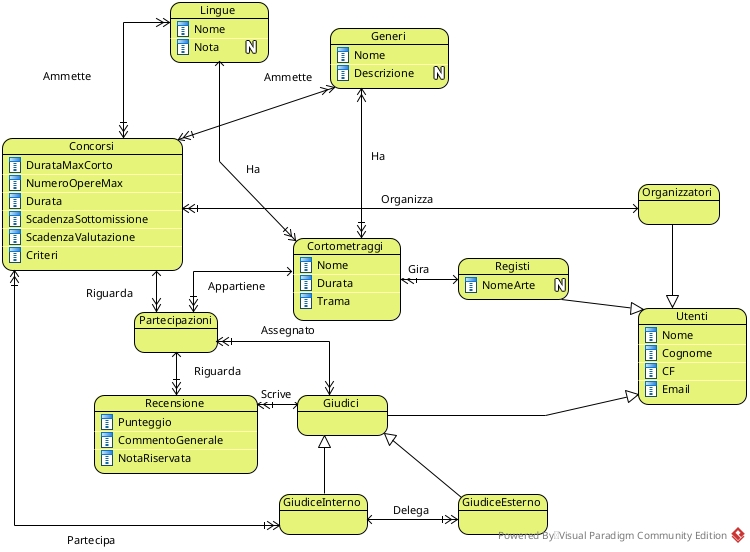
\includegraphics[scale=.5]{ERD_ConCorto.jpg}
\end{center}

\begin{note}
	Al momento della delega da parte di un \textbf{Giudice interno} di un \textbf{Giudice esterno}, quest'ultimo viene inserito nel database e viene assegnato alla valutazione di una determinata \textbf{partecipazione} scelta dal delegante.
\end{note}

\begin{note}
	Al momento dell'inserimento della \textbf{partecipazione} di un \textbf{cortometraggio} ad un \textbf{concorso}, vanno controllati i limiti imposti dall'\textbf{organizzatore} (\textit{DurataMaxCorto}, \textit{NumeroOpereMax}, lingue e generi accettati).
\end{note}

\subsection{Vincoli}
\subsubsection{Interrelazionali}
I vincoli interrelazionali sono:
\begin{itemize}
	\item Un giudice non può giudicare più di un cortometraggio per regista
	\item Un cortometraggio ha 3 giudici assegnati
	\item Un giudice può delegare al più un esterno per ogni concorso
	\item Un organizzatore non può partecipare come regista ad un concorso che organizza
	\item Un giudice può scrivere una sola recensione per cortometraggio per ogni concorso
	\item Se un giudice ha delegato la valutazione non può scrivere la recensione per il cortometraggio che ha delegato
\end{itemize}
\subsubsection{Intrarelazionali}
I vincoli intrarelazionali sono:
\begin{itemize}
	\item \textbf{Generi}: \textit{Descrizione} è NULLABLE
	\item \textbf{Lingue}: \textit{Nota} è NULLABLE
	\item \textbf{Concorsi}: \textit{DurataMaxCorto} $> 0$, \textit{NumeroOpereMax} $>0$, \textit{Durata} $>0$, \textit{ScadenzaSottomissione} $<$ \textit{ScadenzaValutazione}
	\item \textbf{Cortometraggi}: \textit{Durata} $>0$
	\item \textbf{Recensione}: $0\leq$\textit{Punteggio} $\leq 5$
	\item \textbf{Utenti}: \textit{Email} deve rispettare la seguente REGEX
	\begin{lstlisting}[language=Javascript]
		/^[\w-\.]+@([\w-]+\.)+[\w-]{2,4}$/g
	\end{lstlisting}
	\textit{CF} deve rispettare la seguente REGEX
	\begin{lstlisting}[language=Javascript]
		/^(?:[A-Z][AEIOU][AEIOUX]|[AEIOU]X{2}|[B-DF-HJ-NP-TV-Z]{2}[A-Z]){2}(?:[\dLMNP-V]{2}
		(?:[A-EHLMPR-T](?:[04LQ][1-9MNP-V]|[15MR][\dLMNP-V]|[26NS][0-8LMNP-U])|[DHPS]
		[37PT][0L]|[ACELMRT][37PT][01LM]|[AC-EHLMPR-T][26NS][9V])|(?:[02468LNQSU][048LQU]
		|[13579MPRTV][26NS])B[26NS][9V])(?:[A-MZ][1-9MNP-V][\dLMNP-V]{2}|[A-M][0L]
		(?:[1-9MNP-V][\dLMNP-V]|[0L][1-9MNP-V]))[A-Z]$/i
	\end{lstlisting}
	\item \textbf{Registi}: \textit{NomeArte} è NULLABLE
\end{itemize}
Dove non specificato, l'attributo è NON NULLABLE.

\newpage
\section{Schema logico relazionale}
\begin{center}
	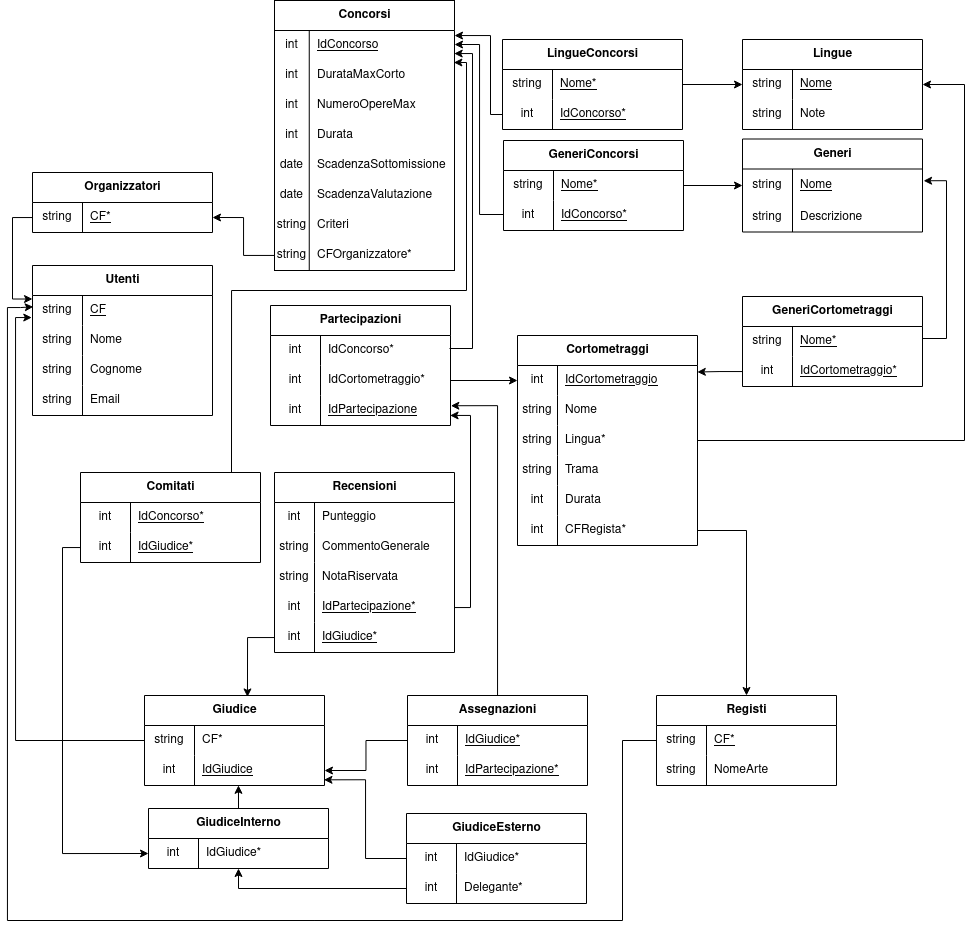
\includegraphics[scale=0.45]{BD0525_logico}
\end{center}

\subsection{Dipendenze funzionali}
Tutte le relazioni $R$ con attributi $A_1, \ldots, A_n$ chiave $K \notin A_1, \ldots, A_n$ hanno una sola dipendenza funzionale del tipo $K \to A_1, \ldots, A_n$.

\subsection{BCNF}
Tutte le relazioni sono in BCNF.

\newpage
\section{Interrogazioni in SQL}
Di seguito le sei interrogazioni richieste:
\begin{enumerate}
	\item[a.] Trova i nomi e le email degli utenti che sono registi e hanno diretto un cortometraggio di durata superiore a 25 minuti.
	\begin{lstlisting}[language=SQL]
		SELECT U.Nome, U.Email
		FROM Utenti U
		JOIN Registi R ON U.CF = R.CF
		JOIN Cortometraggi C ON R.CF = C.CFRegista
		WHERE C.Durata > 25;
	\end{lstlisting}
	\item[b.] Trova i concorsi con più di due lingue ammesse e con una durata massima inferiore a 120 giorni ordinati per numero di lingue in ordine decrescente.
	\begin{lstlisting}[language=SQL]
		SELECT C.IdConcorso, C.Durata, COUNT(L.Nome) AS NumeroLingue
		FROM Concorsi C
		JOIN LingueConcorsi LC ON C.IdConcorso = LC.IdConcorso
		JOIN Lingue L ON L.Nome = LC.Nome
		WHERE C.Durata < 120
		GROUP BY C.IdConcorso, C.Durata
		HAVING COUNT(L.Nome) > 2
		ORDER BY NumeroLingue DESC;
	\end{lstlisting} 
	\item[c.] Trova i generi di cortometraggi lunghi almeno 20 minuti che hanno una durata media superiore a 22 minuti, raggruppati per genere.
	\begin{lstlisting}[language=SQL]
		SELECT G.Nome, AVG(C.Durata) AS DurataMedia
		FROM GeneriCortometraggi GC
		JOIN Generi G ON G.Nome = GC.Nome
		JOIN Cortometraggi C ON C.IdCortometraggio = GC.IdCortometraggio
		WHERE C.Durata > 20
		GROUP BY G.Nome
		HAVING AVG(C.Durata) > 22;
	\end{lstlisting} 
	\item[d.] Trova i nomi dei cortometraggi che hanno almeno una recensione con punteggio superiore a 2.
	\begin{lstlisting}[language=SQL]
		SELECT C.Nome
		FROM Cortometraggi C
		WHERE EXISTS (
			SELECT *
			FROM Recensioni R
			JOIN Partecipazioni P ON R.IdPartecipazione = P.IdPartecipazione
			WHERE P.IdCortometraggio = C.IdCortometraggio AND R.Punteggio > 2
		);
	\end{lstlisting} 
	\item[e.] Trova i nomi dei concorsi in cui tutti i cortometraggi partecipanti hanno una durata inferiore a 30 minuti.
	\begin{lstlisting}[language=SQL]
		SELECT C.IdConcorso
		FROM Concorsi C
		WHERE NOT EXISTS (
		SELECT *
			FROM Partecipazioni P
			JOIN Cortometraggi CM ON P.IdCortometraggio = CM.IdCortometraggio
			WHERE P.IdConcorso = C.IdConcorso AND CM.Durata >= 30
		);
	\end{lstlisting}
	\newpage
	\item[f.] Trova i giudici che hanno assegnato un punteggio superiore alla media dei punteggi di tutti i giudici.
	\begin{lstlisting}[language=SQL]
		SELECT G.IdGiudice, G.CF
		FROM Giudici G
		WHERE EXISTS (
			SELECT *
			FROM Recensioni R
			WHERE R.IdGiudice = G.IdGiudice AND R.Punteggio > (
				SELECT AVG(Punteggio) 
				FROM Recensioni
			)
		);
	\end{lstlisting} 
\end{enumerate}

\newpage
\section{Piani di accesso}
\begin{enumerate}
	\item[I.] Piani di accesso \textbf{logico}
	\begin{figure}[!h]
		\centering
		\begin{minipage}{\textwidth}
			\centering
			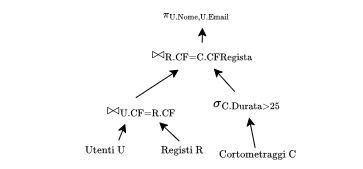
\includegraphics[scale=0.7]{1a.png}
			\captionof{figure}{Query \textit{a}}
		\end{minipage}
		\begin{minipage}{\textwidth}
			\centering
			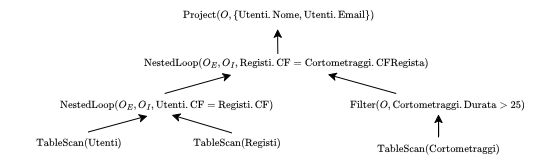
\includegraphics[scale=0.7]{1b.png}
			\captionof{figure}{Query \textit{b}}
		\end{minipage}
		\begin{minipage}{\textwidth}
			\centering
			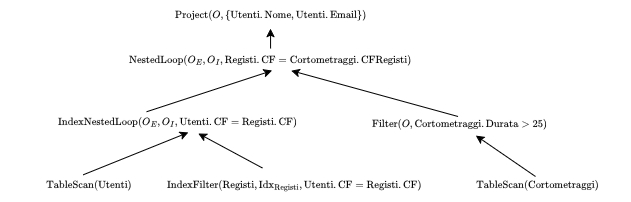
\includegraphics[scale=0.65]{1c.png}
			\captionof{figure}{Query \textit{c}}
		\end{minipage}
	\end{figure}
	
	\newpage
	\item[II.] Piani di accesso \textbf{fisico} senza uso di indici
	\begin{figure}[!h]
		\centering
		\begin{minipage}{\textwidth}
			\centering
			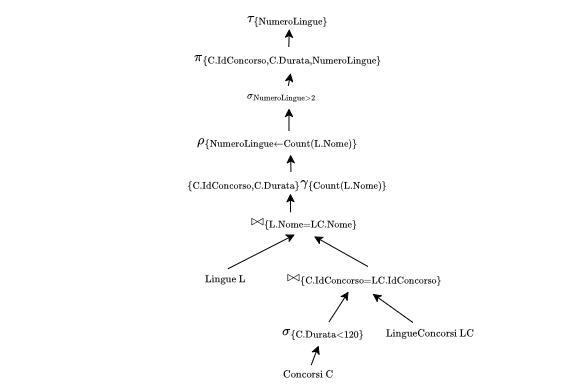
\includegraphics[scale=0.7]{2a.png}
			\captionof{figure}{Query \textit{a}}
		\end{minipage}\\
		\begin{minipage}{\textwidth}
			\centering
			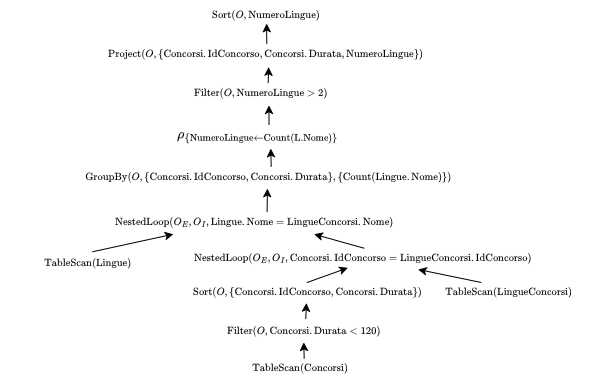
\includegraphics[scale=0.7]{2b.png}
			\captionof{figure}{Query \textit{b}}
		\end{minipage}
	\end{figure}
	\begin{figure}[!h]
		\centering
		\begin{minipage}{\textwidth}
			\centering
			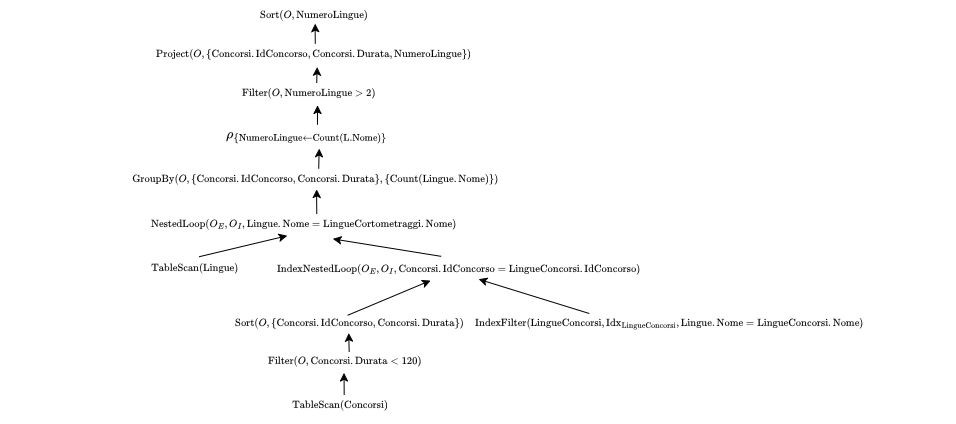
\includegraphics[scale=0.55]{2c.png}
			\captionof{figure}{Query \textit{c}}
		\end{minipage}
	\end{figure}
	
	\newpage
	\item[III.] Piani di accesso \textbf{fisico} con uso di indici
	\begin{figure}[!h]
		\centering
		\begin{minipage}{\textwidth}
			\centering
			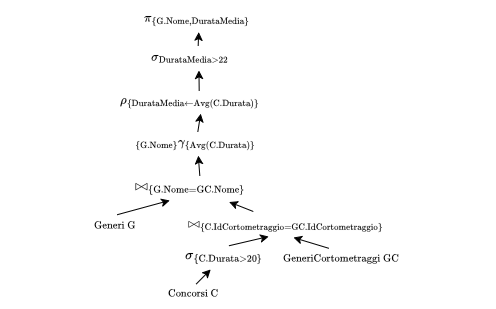
\includegraphics[scale=0.7]{3a.png}
			\captionof{figure}{Query \textit{a}}
		\end{minipage}\\
	\end{figure}
	\begin{figure}[!h]
		\centering
		\begin{minipage}{\textwidth}
			\centering
			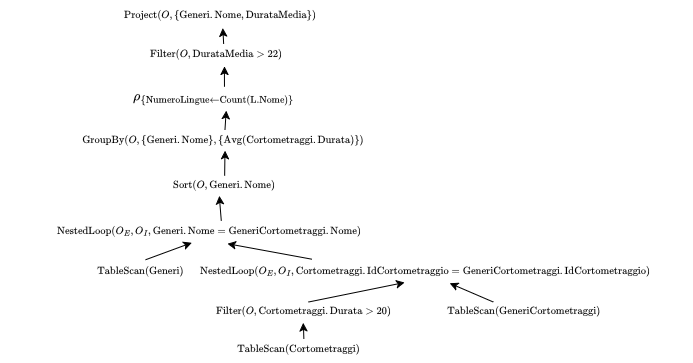
\includegraphics[scale=0.7]{3b.png}
			\captionof{figure}{Query \textit{b}}
		\end{minipage} \hspace{50pt}
		\begin{minipage}{\textwidth}
			\centering
			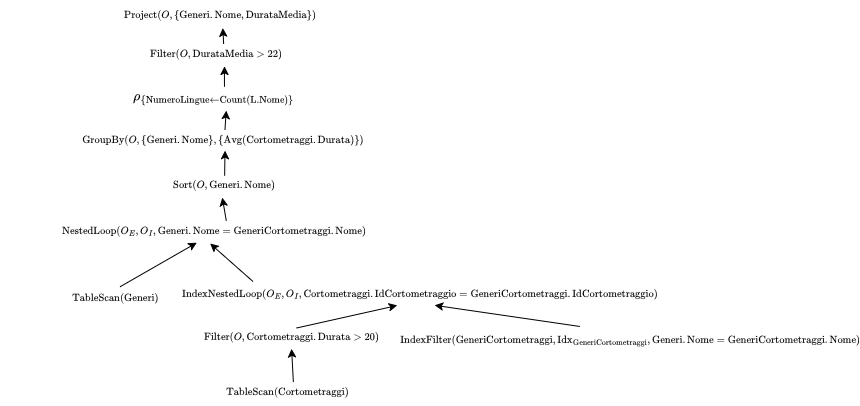
\includegraphics[scale=0.45]{3c.png}
			\captionof{figure}{Query \textit{c}}
		\end{minipage}
	\end{figure}
\end{enumerate}
\input{data}
\input{visualization}
\input{pca}
\input{anomalies}
\input{clustering}
% !TeX spellcheck = en_US
\newpage
\section{Correlation}
This data science method finds the level of correlation between two data modalities and how predictable they are from each other.

\subsection{Pearson's Correlation}
Given a dataset $(x_i, y_i)^N_{i=1}$ with each instance $i$ having two associated features $x_i$ and $y_i$. Let $\mu_x = \mathbb{E}[x]$ and $\mu_y = \mathbb{E}[y]$ be the dataset \textbf{means} for the two features. The Pearson's correlation is:
\begin{equation}
	\rho = \frac{\overbrace{\mathbb{E}[(x-\mu_x)(y-\mu_y)]}^{\sigma_{xy}}}{\underbrace{\sqrt{\mathbb{E}[(x-\mu_x)^2]}}_{\sigma_x} \cdot \underbrace{\sqrt{\mathbb{E}[(y-\mu_y)^2]}}_{\sigma_y}} \qquad\qquad \rho \in [-1,1]
\end{equation}
A value of $1$ indicates correlation, $-1$ negative correlation and $0$ decorrelation.

\subsubsection{Mutual predictability}
\begin{wrapfigure}[5]{r}{4cm}
	\vspace{-1.5cm}
	\begin{center}
		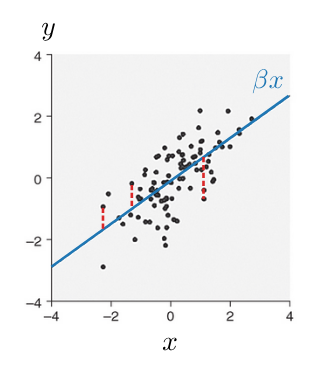
\includegraphics[width=4cm]{pearson}
	\end{center}
\end{wrapfigure}
Lets assume that the data is \textbf{centered}, $\mu_x = \mu_y = 0$, and build a homogeneous linear model that predicts $x$ from $y$ minimizing the square error:
\begin{align*}
	\arg &\min_\beta \mathbb{E}[(y-\beta x)^2]\\
	& = \arg\min_\beta \mathbb{E}[\beta^2x^2 - 2\beta yx]\\
	& = \arg\min_\beta \beta^2\sigma^2_x - 2\beta\sigma_{xy}
\end{align*}
This is a \textbf{convex optimization problem} with solution found at
\begin{equation*}
	\frac{\partial}{\partial\beta}(\beta^2\sigma^2_x - 2\beta\sigma_{xy})=0
\end{equation*}
which gives us the closed form $\beta = \frac{\sigma_{xy}}{\sigma^2_x}$, which injected in the \textit{error function} gives us the error at the optimum, or some measure of predictivity of $y$ from $x$:
\begin{align*}
	\min_\beta & \mathbb{E}[(y - \beta x)^2]\\
	& = \mathbb{E}[(y-\frac{\sigma_{xy}}{\sigma^2_x})^2]\\
	& = \mathbb{E}[y^2] - 2\frac{\sigma_{xy}}{\sigma^2_x} \cdot \mathbb{E}[xy] + \bigg(\frac{\sigma_{xy}}{\sigma^2_x}\bigg)^2 \cdot \mathbb{E}[x^2]\\
	& = \sigma_y ^ 2 - \frac{\sigma_{xy}^2}{\sigma^2_x}\\
	& = \sigma_y ^ 2 \cdot \bigg(1-\bigg(\underbrace{\frac{\sigma_{xy}}{\sigma_x\sigma_y}}_\rho\bigg)^2\bigg)
\end{align*}
Therefore, we have that $\min_\beta \mathbb{E}[(y - \beta x)^2] = \sigma_y^2\cdot (1-\rho^2)$ and $\min_\beta \mathbb{E}[(\beta y - x)^2] = \sigma_x \cdot (1-\rho^2)$, hence there is a \textbf{direct relation} between Pearson's Correlation and mutual predictability

\newpage
\subsection{Canonical Correlation Analysis}
With multivariate data (e.g. images and text, which are composed of multiple features and words) we need to generalize the correlation to modalities of more than one dimension.
\begin{center}
	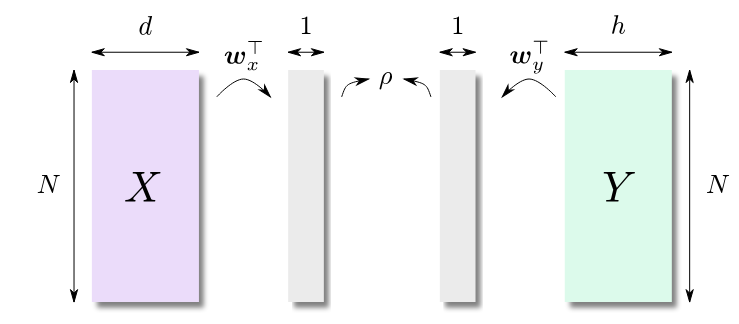
\includegraphics[scale=.3]{cca}
\end{center}
Let $\mathbf{x} \in \mathbb{R}^d$ be the first modality and $\mathbf{y} \in \mathbb{R}^h$ the second one. We want to find the projections $\mathbf{w}_x \in \mathbb{R}^d$ and $\mathbf{w}_y \in \mathbb{R}^h$ of the two modalities in which the Pearson's Correlation is maximized:
\begin{equation*}
	\arg\max_\mathbf{w} \text{Corr}(\mathbf{w}_x^\top \mathbf{x}, \mathbf{w}_y^\top \mathbf{y})
\end{equation*}
\begin{note}
	Since Pearson's Correlation is invariant to the scale of the data, the vectors $\mathbf{w}_x$ and $\mathbf{w}_y$ don't need to be constrained to be e.g. of unit norm.
\end{note}

The correlation can be rewritten as
\begin{align}
	\begin{split}
		\text{Corr}&(\mathbf{w}_x^\top, \mathbf{x}, \mathbf{w}_y^\top \mathbf{y}) \\
		& = \frac{\mathbb{E}[(\mathbf{w}_x^\top(\mathbf{x}-\mathbf{\mu}_x) \cdot  (\mathbf{w}_y^\top(\mathbf{y}-\mathbf{\mu}_y)))]}{\sqrt{\mathbb{E}[(\mathbf{w}_x^\top(\mathbf{x}-\mathbf{\mu}_x))^2]} \cdot \sqrt{\mathbb{E}[(\mathbf{w}_y^\top(\mathbf{y}-\mathbf{\mu}_y))^2]}} \\
		& = \frac{\mathbf{w}_x^\top C_{xy}\mathbf{w}_y}{\sqrt{\mathbf{w}^\top_x C_{xx}\mathbf{w}_x} \cdot \sqrt{\mathbf{w}^\top_y C_{yy}\mathbf{w}_y}} \label{eq:cca}
	\end{split}
\end{align}
where
\begin{align*}
	& C_{xy} = \mathbb{E}[(\mathbf{x}-\mathbf{\mu}_x)(\mathbf{y}-\mathbf{\mu}_y)^\top] \\
	& C_{xx} = \mathbb{E}[(\mathbf{x}-\mathbf{\mu}_x)(\mathbf{x}-\mathbf{\mu}_x)^\top] \\
	& C_{yy} = \mathbb{E}[(\mathbf{y}-\mathbf{\mu}_y)(\mathbf{y}-\mathbf{\mu}_y)^\top]
\end{align*}
are cross-covariance and auto-covariance matrices that can be precomputed. Since the optimum of the problem (as seen in the rewriting of correlation) is specified up to a scaling of $\mathbf{w}_x$ and $\mathbf{w}_y$, we can force a particular scale to get a simpler optimization. In particular we can reformulate it as a \textbf{standard quadratic optimization problem} with quadratic constraints:
\begin{align*}
	\arg \max_\mathbf{w} \mathbf{w}^\top_x C_{xy}\mathbf{w}_y \qquad \text{such that} \qquad & \mathbf{w}_x^\top C_{xx}\mathbf{w}_x = 1 \\
	& \mathbf{w}_y^\top C_{yy}\mathbf{w}_y = 1
\end{align*}
We can then obtain a closed form solution through the Lagrange multipliers method, which is the first eigenvector with highest eigenvalue of the generalized eigenvalue problem:
\begin{equation}
	\begin{bmatrix}
		0 & C_{xy} \\
		C_{yx} & 0
	\end{bmatrix} \begin{bmatrix}
	\mathbf{w}_x \\ \mathbf{w}_y
	\end{bmatrix} = \lambda \begin{bmatrix}
	C_{xx} & 0 \\
	0 & C_{yy} 
	\end{bmatrix} \begin{bmatrix}
	\mathbf{w}_x \\ \mathbf{w}_y
	\end{bmatrix}
\end{equation}
With the eigenvalue $\lambda$ representing the correlation $\rho$ of data in the two projected spaces.
\newpage
\subsubsection{High Dimensions}
CCA generalized problem may be too expensive to solve if $d$ is large because it involves the eigendecomposition of matrices of size $d \times d$. To solve this, we force the solution to be a weighted combination of the data:
\begin{align*}
	& \mathbf{w}_x = \sum_{i=1}^{N} (\mathbf{x}_i-\mu_x)\alpha_{x,i} = \tilde{X}\mathbf{\alpha}_x \qquad\qquad \mathbf{\alpha}_x \in \mathbb{R}^N\\
	& \mathbf{w}_y = \sum_{i=1}^{N} (\mathbf{y}_i-\mu_y)\alpha_{y,i} = \tilde{Y}\mathbf{\alpha}_y \qquad\qquad \mathbf{\alpha}_y \in \mathbb{R}^N
\end{align*}
with $\tilde{X}$ and $\tilde{Y}$ being two matrices containing the \textbf{centered} data. Therefore we have that CCA with $\mathbf{\alpha}$ injected becomes:
\begin{align*}
	\arg \max_\mathbf{\alpha} \overbrace{\mathbf{\alpha}_x^\top\tilde{X}^\top}^{\mathbf{w}_x^\top}C_{xy}\overbrace{\tilde{Y}\mathbf{\alpha}_y}^{\mathbf{w}_y} \qquad \text{such that} \qquad & \overbrace{\mathbf{\alpha}_x^\top\tilde{X}^\top}^{\mathbf{w}_x^\top}C_{xx}\overbrace{\tilde{X}\mathbf{\alpha}_x}^{\mathbf{w}_x} = 1 \\
	& \underbrace{\mathbf{\alpha}_y^\top\tilde{Y}^\top}_{\mathbf{w}_y^\top}C_{yy}\underbrace{\tilde{Y}\mathbf{\alpha}_y}_{\mathbf{w}_y} = 1
\end{align*}
Observing that:
\begin{itemize}
	\item $C_{xy} = \frac{1}{N}\tilde{X}\tilde{Y}^\top$
	\item $C_{xx} = \frac{1}{N}\tilde{X}\tilde{X}^\top$
	\item $C_{yy} = \frac{1}{N}\tilde{Y}\tilde{Y}^\top$
\end{itemize}
the objective becomes
\begin{align*}
	\arg\max_\mathbf{\alpha} \mathbf{\alpha}_x^\top \overbrace{\frac{1}{N}\tilde{X}^\top\tilde{X}\tilde{Y}^\top\tilde{Y}}^{Q_{xy}}\mathbf{\alpha}_y \qquad \text{such that} \qquad & \mathbf{\alpha}_x^\top \overbrace{\frac{1}{N}\tilde{X}^\top \tilde{X}\tilde{X}^\top\tilde{X}}^{Q_{xx}} \mathbf{\alpha}_x = 1 \\
	& \mathbf{\alpha}_y^\top \underbrace{\frac{1}{N}\tilde{Y}^\top \tilde{Y}\tilde{Y}^\top\tilde{Y}}_{Q_{yy}} \mathbf{\alpha}_y = 1
\end{align*}
where $Q_{xy}$, $Q_{xx}$ and $Q_{yy}$ are matrices of size $N \times N$ instead of $d \times d$. At this point we have the formulation of the optimization problem that's in the same form as the original CCA but with different matrices and optimization variables
\begin{align}
	\begin{split}
		\arg\max_\mathbf{\alpha} \mathbf{\alpha}_x^\top Q_{xy} \mathbf{\alpha}_y \qquad \text{such that} \qquad & \mathbf{\alpha}_x^\top Q_{xx} \mathbf{\alpha}_x = 1 \\
		& \mathbf{\alpha}_y^\top Q_{yy} \mathbf{\alpha}_y = 1
	\end{split}
\end{align}
and therefore we can use the same framework of Lagrange multipliers to find the solution $\mathbf{\alpha}$ as the leading eigenvector of a generalized eigenvalue problem
\begin{equation}
	\underbrace{
		\begin{bmatrix}
			0 &  Q_{xy} \\
			Q_{yx} & 0
	\end{bmatrix}}_A \begin{bmatrix}
	\mathbf{\alpha}_x \\ \mathbf{\alpha}_y
\end{bmatrix} = \lambda \underbrace{\begin{bmatrix}
	Q_{xx} & 0 \\
	0 & Q_{yy}
	\end{bmatrix}}_{B} \begin{bmatrix}
	\mathbf{\alpha}_x \\ \mathbf{\alpha}_y
\end{bmatrix}
\end{equation}

\begin{note}
	For \textbf{stability} it's useful to add a small diagonal term on the matrix $B$.
\end{note}

\newpage
\subsubsection{Temporal}
If variables are coupled with delays (e.g. medical data from different sources like fMRI and spectrogram of neural activity), simultaneous samples will not be coupled and standard CCA will not find the right solution.\\
The solution is to \textbf{shift} one variable relative to the other and maximize the correlation for a sum over all relative time lags.
\begin{equation}
	\underset{w_x(\tau), w_y}{\text{argmax}} \text{Corr}\bigg(\sum_\tau w_x(\tau)^\top x(t-\tau), w_y^\top y(t)\bigg)
\end{equation}
We can then create $\tilde{X}$ and $\tilde{w}_x$ and obtain:
\begin{equation}
	\underset{w_{\tilde{x}}, w_y}{\text{argmax}} \text{Corr}(\tilde{w}_x^\top \tilde{X}, w_y^\top Y) \qquad\qquad \tilde{X} = \begin{bmatrix}
		X_{\tau_1} \\ X_{\tau_2} \\ \vdots \\ X_{\tau_T}
	\end{bmatrix} \qquad
	\tilde{w}_x = \begin{bmatrix}
		w_x(\tau_1) \\ w_x(\tau_2) \\ \vdots \\ w_x(\tau_T)
	\end{bmatrix}
\end{equation}

\begin{note}
	In case of \textbf{high dimensionality} we can represent $w_x$ as a weighted combination of the data:
	\begin{equation}
		w_x = X\alpha_x
	\end{equation}
\end{note}

\subsection{Nonlinear Correlations}
In situations where we have a negligible (close to $0$) Pearson's Correlation coefficient we can nonlinearly expand $x$ and $y$ and apply CCA to find a correlation in the expanded space.

\begin{example}
	In this case we expand $x$ to $\phi(x)=[x,x^2,x^3]$ and $y$ to $\phi(y)=[y,y^2,y^3]$ and calculate CCA on both of them. The result is:
	\begin{equation*}
		\lambda_1 = 0.86 \qquad\qquad \mathbf{u}_1 = [\underbrace{-0.13, 1.84, 0.15}_{\mathbf{w}_x}, \underbrace{0.09, -1.88, -0.07}_{\mathbf{w}_y}]
	\end{equation*}
	We notice that 
	\begin{equation*}
		\text{Corr}(0+ x^2+0, 0-y^2+0) \approx 0.86
	\end{equation*}
	and that therefore the data is governed by the equation $x^2 = \alpha(-y^2)+\beta$, where setting $\alpha=1$ and $\beta=1$ gives us $x^2+y^2=1$.
	\begin{center}
		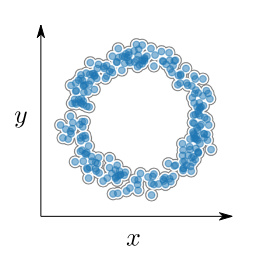
\includegraphics[scale=0.4]{nonlin1}
		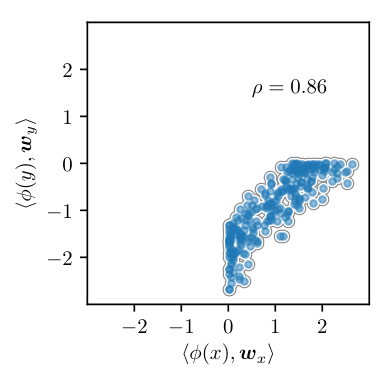
\includegraphics[scale=0.3]{nonlin2}
	\end{center}
\end{example}
% !TeX spellcheck = en_US
\newpage
\section{Prediction}
\subsection{Least Square Regression}
We build a \textbf{model} predicting $y$ from $x$:
\begin{equation}
	f(\mathbf{x}) = \mathbf{w}^\top\mathbf{x} + b
\end{equation}
and we find the model \textbf{parameters} so that prediction errors are minimized. An example could be to minimize the least squared error averaged over all instances:
\begin{equation}
	\min_{\mathbf{w},b} \mathbb{E}[(\mathbf{w}^\top\mathbf{x}+b-y)^2]
\end{equation}
\subsubsection{Centering}
To simplify regression we can \textbf{center} the data by putting $\mathbb{E}[\mathbf{x}] = \mathbf{0}$ and $\mathbb{E}[y]=0$. Then we can show that
\begin{equation}
	\arg \max_b \mathbb{E}[(f(\mathbf{x})-y)^2] = 0
\end{equation}
\begin{demonstration}
	\begin{equation*}
		\frac{\partial}{\partial b} \mathbb{E}[(f(\mathbf{x})-y)^2] = 2\mathbb{E}[(\mathbf{w}^\top\mathbf{x}+b-y)] \overset{\text{def}}{=} 0 \Rightarrow b=0
	\end{equation*}
	\hfill$\square$
\end{demonstration}
This implies that, without loss of accuracy, one can simplify the Least Square Regression problem as finding a homogeneous linear model that minimizes the square error:
\begin{equation}
	f(\mathbf{x}) = \mathbf{w}^\top\mathbf{x}
\end{equation}
\subsubsection{Linear regression}
We can develop it as:
\begin{align}
	\begin{split}
		\xi (\mathbf{w}) & = \mathbb{E}[(f(\mathbf{x}) -y)^2]\\
		& = \mathbb{E}[(\mathbf{w}^\top \mathbf{x}-y)^2] \qquad\qquad\qquad\quad \text{Substitution}\\
		& = \mathbb{E}[\mathbf{w}^\top \mathbf{x}\mathbf{x}^\top\mathbf{w}-2\mathbf{w}^\top\mathbf{x} y + y^2] \quad \text{Square calculation, n.b. } (\mathbf{w}^\top \mathbf{x})^2 = \mathbf{w}^\top \mathbf{x} \mathbf{x}^\top \mathbf{w}\\
		& = \mathbf{w}^\top C_{xx}\mathbf{w} - 2\mathbf{w}^\top C_{xy}+C_{yy} \qquad \text{Linearity and covariance definition}
		\label{eq:linregog}
	\end{split}
\end{align}
Since $C_{xx}$ is positive semi-definite, minimizing $\xi(\mathbf{w})$ is a \textbf{convex optimization problem} and the solution must necessarily have gradient zero:
\begin{equation}
	\nabla\xi(\mathbf{w}) = 2C_{xx}\mathbf{w} - 2C_{xy}=0 \longrightarrow \mathbf{w} = C_{xx}^{-1}C_{xy}
\end{equation}
If we inject this into the objective we get the \textbf{mean square error} at the optimum:
\begin{equation}
	\xi = C_{yy} - C_{yx}C^{-1}_{xx} C_{xy} \label{eq:linreg}
\end{equation}

\paragraph{Non-Invertible $C_{xx}$}
\begin{wrapfigure}[6]{r}{4cm}
\vspace{-.9cm}
\begin{center}
	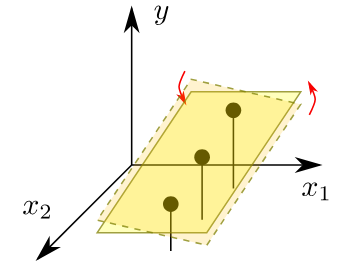
\includegraphics[width=4cm]{lsr}
\end{center}
\end{wrapfigure}
If we have $C_{xx}$ non invertible corresponds to the case  where the data only spans a subspace of $\mathbb{R}^d$. In this case, there are infinitely many possible solutions to the regression problem.\\
To solve this we virtually add some \textbf{noise} $\mathbf{n}$ to the data (adding a diagonal term to the covariance matrix) so that the covariance matrix is now invertible and favors solutions that are flat on directions that are orthogonal to the data.
\begin{align}
	\begin{split}
		C_{xx}^{\text{new}} & = \text{Cov} ( \mathbf{x}+\mathbf{n}, \mathbf{x} + \mathbf{n}) \\
		& = \text{Cov}(\mathbf{x}, \mathbf{x}) + 2 \text{Cov}(\mathbf{x}, m\mathbf{n}) + \text{Cov}(\mathbf{n}, m\mathbf{n})\\
		& = C_{xx}+\sigma_n^2I
	\end{split}
\end{align}
Using the new covariance in the error function \ref{eq:linreg} yields:
\begin{align}
	\begin{split}
		\xi^{\text{new}}&=C_{yy}-C_{yx}(C_{xx}^\text{new})^{-1}C_{xy} \\
		& = C_{yy} - C_{yx}(C_{xx} + \sigma_n^2 I)^{-1}C_{xy} \\
		& = C_{yy} - C_{yx} \bigg(\sum_{j=1}^{d} u_j u_j^\top ( \lambda_j + \sigma_n^2)\bigg)^{-1}C_{xy} \\
		& = C_{yy} - \sum_{j} (C_{yx}u_j)^2 \frac{1}{\lambda_j+\sigma_n^2}
	\end{split}
\end{align}
The larger the noise we inject, the higher the error: wee need just enough to make $C_{xx}$ invertible.

\paragraph{High Dimensions} When $d$ is large, computing and inverting $C_{xx}$ can get really expensive. To manage this, we start from the formulation \ref{eq:linregog} and we assume that an optimal $\mathbf{w}$ is found in the span of the data and we express it as a linear combination of the data $\mathbf{w} = X \mathbf{\alpha}$, where $X$ is a matrix of size $d \times N$ containing the centered data:
\begin{align}
	\begin{split}
		\xi(\mathbf{\alpha}) & = \overbrace{\mathbf{\alpha}^\top X^\top}^{\mathbf{\alpha}^\top}C_{xx}\overbrace{X\mathbf{\alpha}}^{\mathbf{w}} - 2 \overbrace{\mathbf{\alpha}^\top X^\top}^{\mathbf{w}^\top}C_{xy}+C_{yy} \\
		& = \frac{1}{N}\mathbf{\alpha}^\top \underbrace{X^\top XX^\top X}_{Q_x^2}-\frac{2}{N}\mathbf{\alpha}^\top \underbrace{X^\top X}_{Q_x}Y+C_{yy}
	\end{split}
\end{align} 
Since matrices $Q_x^2$ and $Q_x$ are of size $N \times N$ there is no need to compute matrices of size $d \times d$ anymore. Since $\xi(\mathbf{\alpha})$ is convex, we can find the solution where the gradient $\nabla\xi(\mathbf{\alpha}) = \frac{2}{N}Q_x^2\mathbf{\alpha}-\frac{2}{N}W_x Y$is zero:
\begin{equation*}
	\mathbf{\alpha} = (Q_x^2)^{-1}Q_xY = Q_x^{-1}Y
\end{equation*}
And therefore we need to invert only a matrix of size $N \times N$. From this we can then recover the original weight parameter as:
\begin{equation}
	\mathbf{w} = X \mathbf{\alpha}
\end{equation}

\subsubsection{CCA}
Since in the case of linear regression the second modality is \textbf{univariate}, there is no direction to be found in the second modality ($w_y = 1$) and the CCA objective (\ref{eq:cca}) simplifies to:
\begin{equation}
	\rho = \frac{\mathbf{w}_x^\top C_{xy}}{\sqrt{\mathbf{w}^\top_x C_{xx}\mathbf{w}_xC_{yy}}} 
\end{equation}
which can then be reformulated as a constrained optimization problem:
\begin{equation}
	\max_\mathbf{w} \mathbf{w}_x^\top C_{xy} \qquad\text{such that}\qquad \mathbf{w}_x^\top C_{xx}\mathbf{w}_xC_{yy} = 1 \label{eq:ccalsr}
\end{equation}

\paragraph{Weights}
To derive the weights we solve the problem indicated in equation \ref{eq:ccalsr} with Lagrange's Multipliers:
\begin{align*}
	&\mathcal{L}(\mathbf{w}_x, \lambda) = \mathbf{w}_x^\top C_{xy} + \frac{1}{2} \lambda (1-\mathbf{w}_x^\top C_{xx}\mathbf{w}_x C_{yy}) \\
	&\frac{\partial \mathcal{L}}{\partial\mathbf{w}_x} = C_{xy}-\lambda C_{xx}\mathbf{w}_x C_{yy} = 0 \Longrightarrow \mathbf{w}_x = \lambda^{-1}C^{-1}_{xx}C_{xy}C_{yy}^{-1}
\end{align*}
Therefore, setting $\lambda$ in a way that the constraint is satisfied, we get:
\begin{equation}
	\mathbf{w}_x = \frac{C_{xx}^{-1}C_{xy}}{\sqrt{C_{yx}C_{xx}^{-1}C_{xy}C_{yy}}} \label{eq:ccalsrw}
\end{equation}
which is exactly the same direction as the weight of the linear model $\mathbf{w} = C_{xx}^{-1}C_{xy}$.
\paragraph{Objective} To derive the objective we evaluate the CCA objective equation with the solution \ref{eq:ccalsrw}. This gives us the \textbf{correlation coefficient}
\begin{equation*}
	\rho = \mathbf{w}_x^\top C_{xy} = \sqrt{C_{yx}C_{xx}^{-1}C_{xy}C_{yy}^{-1}}
\end{equation*}
From which we can measure the \textbf{explained variance}
\begin{equation}
	C_{yy}\rho^2 = C_{yx}C_{xx}^{-1}C_{xy} \label{eq:cca1}
\end{equation}
which compared to the error of linear regression \ref{eq:linreg} indicates that the CCA objective and Least Square Regression ar related: they form a composition of the total variance.
\begin{equation}
	C_{yy} = C_{yy}\rho^2 + \xi
\end{equation}
This means that maximizing the correlation with CCA and minimizing Square Error achieve both the same objective.

\subsection{Outliers}
Square errors may be very large for data points whose outputs strongly deviate from that of other data points. Those with large prediction errors may be treated as \textbf{outliers} so that the model can focus on the non-outlier part of the data. Reduced sensitivity to those can be achieved by considering absolute deviations instead of squared errors and invariance to small noise can be maintained by introducing a small \textbf{slack} $\epsilon$.
\begin{center}
	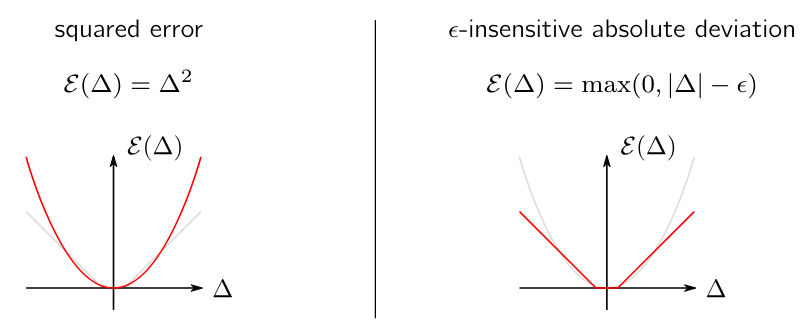
\includegraphics[scale=0.3]{regout}
\end{center}
To do this we replace the square error in the original problem by the $\epsilon$-insensitive absolute deviation and we add a \textbf{penalty term} $\lambda\lvert\lvert \mathbf{w}\rvert\rvert^2$ to favor the flattest solution:
\begin{equation*}
	\min_\mathbf{w} \mathbb{E}[(\mathbf{w}^\top \mathbf{x}-y)^2] \longrightarrow \min_{\mathbf{w},b}[\max(0,\lvert \mathbf{w}^\top x + b -y \rvert -\epsilon)] + \lambda\lvert\lvert \mathbf{w}\rvert\rvert^2
\end{equation*}
\begin{note}
	We have to reintroduce the bias $b$ because we are no longer guaranteed that a solution without it is optimal.
\end{note}

\subsubsection{Support  Vector Regression}
An algorithm that implements this is Support Vector Regression, which takes the form of a quadratic optimization problem with linear constraints. The \textbf{primal} version is:
\begin{align}
	\begin{split}
		\min_{\mathbf{w},b,\mathbf{\xi},\mathbf{\xi^\star}} \frac{1}{2}  \lvert\lvert \mathbf{w}\rvert\rvert^2+C\sum_{i=1}^{N}(\xi_i + \xi_i^\star) \qquad \text{such that} \qquad & \forall_{i=1}^N : \mathbf{w}^\top \mathbf{x}_i + b - y_i \leq \epsilon + \xi_i \\
		& \forall_{i=1}^N : y_i -\mathbf{w}^\top \mathbf{x}_i + b \leq \epsilon + \xi_i \\
		& \xi_i, \xi_i^\star \geq 0
	\end{split}
\end{align}
The \textbf{dual} version is:
\begin{align}
	\begin{split}
		\max_{\alpha, \alpha^\star} -\frac{1}{2}\sum_{ij}(\alpha_i-\alpha_i^\star)(a_j - a_j^\star)\mathbf{x}_i^\top \mathbf{x}_j  \qquad \text{such that} \qquad & \sum_i(a_i - a_i^\star) = 0 \\
		- \varepsilon \sum_i(a_i +a_i^\star) +\sum_i y_i(a_i - a_i^\star)  \qquad \qquad\qquad\qquad& a_i, a_i^\star \in [0, C]
	\end{split}
\end{align}
This algorithm enable the model to be robust to outliers data and to small noise perturbations. Both versions take the form of a quadratic optimization problem with linear constraints. The \textbf{disadvantages} are that SVR has no closed form solution and there is no simpler relation between the objective and statistical measures (e.g. correlation, variance).

\subsection{Difference of means}
Let $\mathbf{x}_1, \ldots, \mathbf{x}_n$ be a dataset and each member is an instance of one the two groups. Let $\mathcal{G}_1$ and $\mathcal{G}_2$ be the set instances of each group.\\
We formulate the problem of \textbf{discriminant learning} as finding a unit-norm vector $\mathbf{w}$ such that the projected data points are maximally different between the two groups on average:
\begin{align}
	\begin{split}
		\max_{\mathbf{w}} &\frac{1}{\lvert \mathcal{G}_1\rvert \lvert \mathcal{G}_2 \rvert} \sum_{i \in \mathcal{G}_1} \sum_{j \in \mathcal{G}_2} (\mathbf{w}^\top \mathbf{x}_i- \mathbf{w}^\top\mathbf{x}_j) \\
		& = \max_{\mathbf{w}} \frac{1}{\lvert \mathcal{G}_1\rvert \lvert \mathcal{G}_2 \rvert} \mathbf{w}^\top \bigg(\lvert \mathcal{G}_2\rvert\sum_{i \in \mathcal{G}_1} \mathbf{x}_i - \lvert \mathcal{G}_1 \rvert \sum_{j \in \mathcal{G}_2} \mathbf{x}_i\bigg) \\
		& = \max_{\mathbf{w}} \mathbf{w}^\top \bigg(\frac{1}{\lvert \mathcal{G}_1\rvert}\sum_{i \in \mathcal{G}_1} \mathbf{x}_i - \frac{1}{\lvert \mathcal{G}_2 \rvert }\sum_{j \in \mathcal{G}_2} \mathbf{x}_i\bigg) \\
		& = \max_{\mathbf{w}} \mathbf{w}^\top (\mu_1 - \mu_2)
	\end{split}
\end{align}
and the unit-norm vector $\mathbf{w}$ that maximizes this objective is the difference of means:
\begin{equation}
	\mathbf{w} = \frac{(\mu_1 -\mu_2)}{\lvert\lvert \mu_1-\mu_2\rvert\rvert}
\end{equation}
\subsubsection{Fisher Discriminant}
Sometimes a better model can be achieved by rotating the projection, increasing their \textbf{separability}.
\begin{center}
	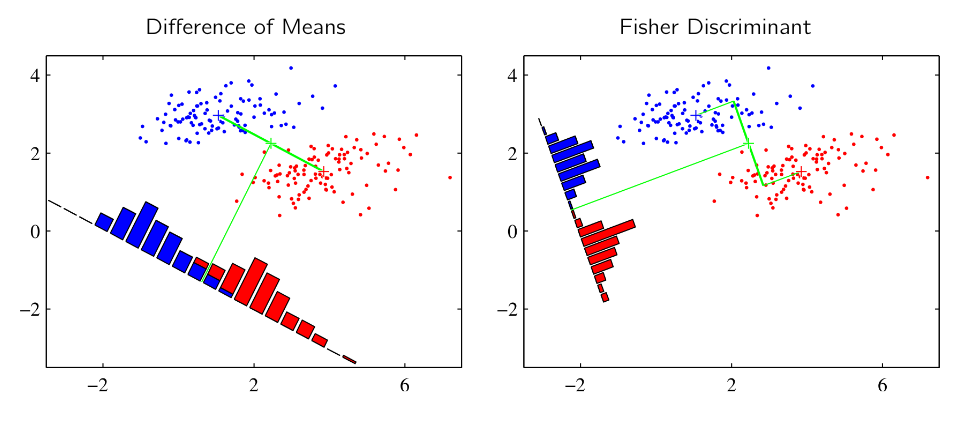
\includegraphics[scale=.4]{fischer}
\end{center}
To do this, in addition to maximizing the separation between class means in projected space, the Fisher Discriminant also \textbf{reduces the within group scatter}:
\begin{equation}
	s_k(\mathbf{2}) = \sum_{i \in \mathcal{G}_k} (\mathbf{w}^\top (\mathbf{x}_i - \mu_k))^2
\end{equation}
Then we define the new \textbf{objective} as:
\begin{equation}
	\max_{\mathbf{w}} \frac{\mathbf{w}^\top (\mu_1 - \mu_2)}{\sqrt{s_1(\mathbf{w}) + s_2(\mathbf{w})}}
\end{equation}
Since the \textbf{scatter terms} have the quadratic form
\begin{equation*}
	s_k(\mathbf{w}) = \mathbf{w}^\top \underbrace{\sum_{i \in \mathcal{G}_k} (\mathbf{x}_i - \mu_k) (\mathbf{x}_i - \mu_k)^\top\mathbf{w}}_{S_k}
\end{equation*}
we can rewrite the objective as
\begin{equation}
	\max_{\mathbf{w}} \frac{\mathbf{w}^\top (\mu_1 - \mu_2)}{\sqrt{\mathbf{w}^\top (S_1 + S_2) \mathbf{w}}}
\end{equation}
and since the objective is invariant to a rescaling of $\mathbf{w}$, we can use instead this constrained optimization problem:
\begin{equation}
	\max_{\mathbf{w}} \mathbf{w}^\top (\mu_1 - \mu_2) \qquad \text{such that} \qquad \frac{1}{2} \mathbf{w}^\top (S_1+ S_2) \mathbf{w} = 1
\end{equation}
Which can then be solved with the Lagrange's Multipliers method:
\begin{equation*}
	\mathbf{w} = (S_1 + S_2)^{-1}(\tau_1 - \tau_2)
\end{equation*}
\paragraph{Connection to CCA}
The Fisher Discriminant  can be seen as a special case of CCA: interpretation as a projection that maximizes correlation between input and output. To demonstrate this we develop the cross-covariance between $\mathbf{x}$ and $y$  as:
\begin{align*}
	C_{xy} & = \frac{1}{N} \sum_{i=1}^{N} (\mathbf{x}_i -\mu_x)(y_i - \mu_y) \\
	& = \frac{1}{N} \bigg[\sum_{i \in \mathcal{G}_1}(\mathbf{x}_i -\mu_x)(1 - \mu_y) + \sum_{i \in \mathcal{G}_2}(\mathbf{x}_i -\mu_x)(-1 - \mu_y)\bigg] \\
	& = \frac{1}{N} \bigg[\sum_{i \in \mathcal{G}_1}(\mathbf{x}_i -\mu_x) - \sum_{i \in \mathcal{G}_2}(\mathbf{x}_i -\mu_x) + \underbrace{\sum_{i=1}^{N}(\mathbf{x}_i - \mu_x)}_0 \cdot (-\mu_y)\bigg] \\
	& = \frac{\lvert \mathcal{G}_1 \rvert}{N} (\mu_1 -\mu_x) - \frac{\lvert \mathcal{G}_2\rvert}{N}(\mu_2 - \mu_x) \\
	& = \frac{2\lvert\mathcal{G}_1\rvert\lvert \mathcal{G}_2\rvert}{N^2}(\mathcal{\mu}_1 - \mu_2)
\end{align*}
and since $y$ follows essentially a Bernoulli distribution, we get:
\begin{equation}
	C_{yy} = \frac{4\lvert\mathcal{G}_1\rvert\lvert \mathcal{G}_2\rvert}{N^2}
\end{equation}
We can the inject these two found covariances into \ref{eq:cca1} and we get:
\begin{align*}
	\rho^2 & = C_{yx}C_{xx}^{-1}C_{xy}C_{yy}^{-1}\\
	& = \frac{2\lvert\mathcal{G}_1\rvert\lvert \mathcal{G}_2\rvert}{N^2}(\mu_1 - \mu_2)C_{xx}^{-1}\frac{2\lvert\mathcal{G}_1\rvert\lvert \mathcal{G}_2\rvert}{N^2}(\mu_1 - \mu_2)\frac{N^2}{4\lvert\mathcal{G}_1\rvert\lvert \mathcal{G}_2\rvert} \\
	& = \frac{\lvert\mathcal{G}_1\rvert\lvert \mathcal{G}_2\rvert}{N^2}(\mu_1 - \mu_2)^\top C_{xx}^{-1}(\mu_1 - \mu_2)
\end{align*}
and substituting to \ref{eq:ccalsrw} we get
\begin{align*}
	\mathbf{w}_x & = \frac{C_{xx}^{-1}C_{xy}}{\sqrt{C_{yx}C_{xx}^{-1}X_{xy}}} \\
	& = \frac{C_{xx}^{-1}\frac{2\lvert\mathcal{G}_1\rvert\lvert \mathcal{G}_2\rvert}{N^2}(\mu_1 - \mu_2)}{\sqrt{\ldots}}\\
	& \propto C_{xx}^{-1}(\mu_1 - \mu_2)
\end{align*}
\begin{proposition}
	CCA and the Fisher vector point to the same direction
	\begin{equation}
		(S_1 + S_2)^{-1}(\mu_1 - \mu_2) \propto C_{xx}^{-1}(\mu_1 - \mu_2)
	\end{equation}
\end{proposition}
\begin{demonstration}
	\begin{align*}
		C_{xx} & = \frac{1}{N} \sum_{i=1}^{N} (x_1 - \mu)(\mathbf{x}_i - \mu)^\top \\
		& = \frac{1}{N} \sum_{k \in \{1,2\}}\sum_{i \in \mathcal{G}_k} (\mathbf{x}_i - \mu) (\mathbf{x}_i \mu)^\top \\
		& = \frac{1}{N} \sum_{k \in \{1,2\}}\sum_{i \in \mathcal{G}_k} (\mathbf{x}_i -\mu_k + \mu_k -\mu)(\mathbf{x}_i - \mu_k + \mu_k -\mu)^\top \\
		& = \bigg(\frac{1}{N} \underbrace{\sum_{k \in \{1,2\}}\sum_{i \in \mathcal{G}_k} (\mathbf{x}_i-\mu_k)(\mathbf{x}_i - \mu_k)^\top}_{S_1 + S_2}\bigg) + \alpha \cdot (\mu_1 - \mu_2)(\mu_1 - \mu_2)^\top + 0
	\end{align*}
	Then, using the identity $(A + \mathbf{b}\mathbf{b}^\top)^{-1} \mathbf{b} \propto A^{-1}\mathbf{b}$ we get that
	\begin{equation*}
		C_{xx}^{-1}(\mu_1 - \mu_2) \propto (S_1 + S_2)^{-1} (\mu_1 - \mu_2)
	\end{equation*}
	\hfill $\square$
\end{demonstration}

\subsection{Support Vector Machine}
Fisher Discriminant is \textbf{strongly affected} by the presence of \textbf{outliers} and may underestimate how predictable group membership is. To solve this problem, we focus on the \textbf{separation between the two groups} rather than their distribution and implement a mechanism that's robust to outliers.\\

To do that we learn a \textbf{hyperplane} that separates the two groups, called the \textbf{Perceptron}. Among all hyperplanes, the SVM chooses the one with the largest margin from the data points.\\
The SVM penalizes absolute deviations instead of square errors to allow for outliers. Therefore, the optimization problem (\textbf{primal problem}) is:
\begin{equation}
	\min_{\mathbf{w},b, \xi} \frac{1}{2} \lvert\lvert \mathbf{w} \rvert\rvert ^2 + C \sum_{i=1}^{N} \xi_i \qquad\text{such that} \qquad \forall_{i=1}^N : (\mathbf{w}^\top \mathbf{x}_i+b) \cdot y_i \geq 1-\xi_i \qquad \xi_i \geq 0
\end{equation}

\subsubsection{Dual problem}
When $d\gg N$ we can use the dual formulation:
\begin{equation}
	\max_\alpha \sum_{i=1}^{N}\alpha_i - \frac{1}{2} \sum_{i=1}^{N} \sum_{j=1}^{N} \alpha_i \alpha_jy_iy_j\mathbf{x}_i^\top \mathbf{x}_j \qquad \text{such that} \qquad \sum_{i}\alpha_i y_i = 0 \qquad \alpha_i \in [0, C]
\end{equation}
\subsubsection{Pros and cons}
SVM has a \textbf{better separation of groups} that Fisher discriminant for general data, it's more \textbf{robust to outliers} enabled by slack variables $\xi_i$ and has a \textbf{convex formulation}, meaning that is guaranteed to converge to the minimum of the objective.\\

On the other hand is \textbf{less suitable} than Fisher Discriminant if we care about within-group homogeneity in projected space, has \textbf{no closed-form solution} and it's not connected to CCA, meaning there is \textbf{no interpretation as maximizing correlation}.
% !TeX spellcheck = en_US
\newpage
\section{Reproducibility}
Most computer based experiments are \textbf{repeatable} while the result of an experiment is \textbf{reproducible} if it's not affected substantially by a limited perturbation of the setup.
\begin{center}
	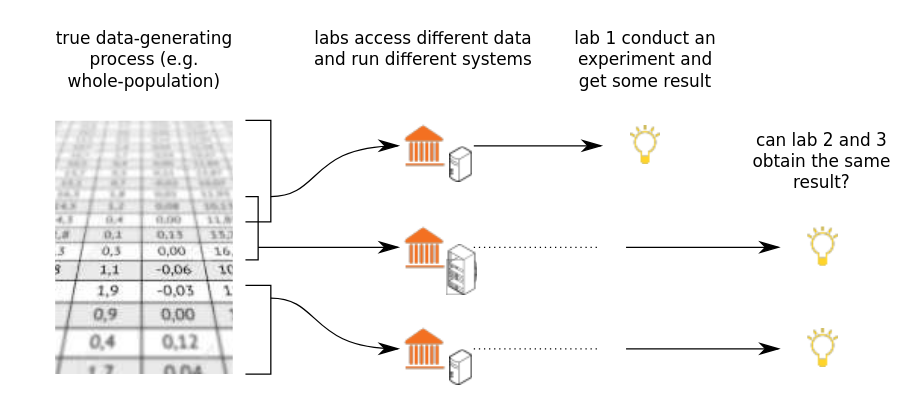
\includegraphics[scale=.4]{reprod}
\end{center}

\subsection{Testing}
\subsubsection{Holdout}
\begin{wrapfigure}[6]{r}{7cm}
	\vspace{-1.3cm}
	\begin{center}
		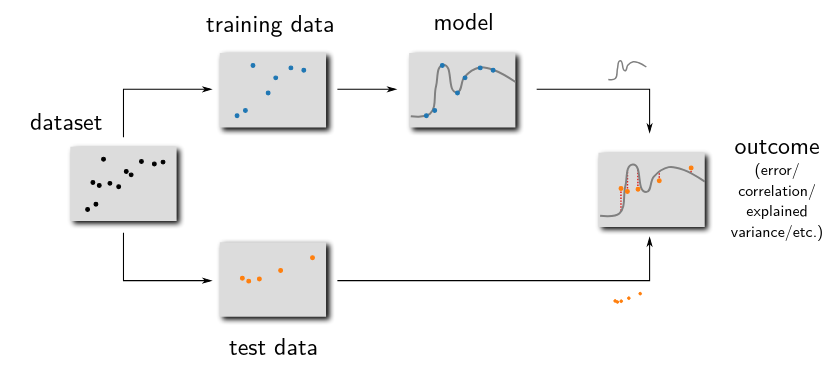
\includegraphics[width=7cm]{holdout}
	\end{center}
\end{wrapfigure}
The idea behind this procedure is to artificially simulate the scenario of another lab reproducing the experiment by randomly partitioning  the available data into \textbf{training} and \textbf{test}. The learning is done on the training data  and the report and results on the test one.

\begin{example}[PCA]
	In the PCA we learn the first principal component $\mathbf{u}_1$ on the \textit{training} data:
	\begin{align*}
		& C_{\text{train}} = \text{Cov}(X_{\text{train}}, X_{\text{train}}) &\text{(estimate the covariance)}\\
		& \mathbf{u}_1 = \arg\max_\mathbf{u} \mathbf{u}^\top C_\text{train} \mathbf{u} & \text{(extract the PCA-1 direction)}
	\end{align*}
	And then we measure the variance explained by $\mathbf{u}_1$ on the \textit{test} data:
	\begin{align*}
		& C_\text{test} = \text{Cov}(X_\text{test}, X_\text{test}) & \text{(estimate the covariance)} \\
		& \lambda_\text{test} = \mathbf{u}_1^\top C_\text{test} \mathbf{u}_1 & \text{(compute the explained variance)}
	\end{align*}
\end{example}

\begin{example}[Least Square Regression]
	In Least Square Regression we train the regression model on the \textit{training} data:
	\begin{align*}
		& C_{xx} = \text{Cov}(X_\text{train}, X_\text{train}) & \text{(estimate the auto-covariance)} \\
		& C_{xy} = \text{Cov}(X_\text{train}, Y_\text{train}) & \text{(estimate the cross-covariance)} \\
		& \mathbf{w} = C^{-1}_{xx}C_{xy} \\
		&b = \mathbb{E}[Y_\text{train}] - \mathbf{w}^\top \mathbb{E}[X_\text{train}]
	\end{align*}
	And then we evaluate the error of the model $(\mathbf{w}, b)$ on the \textit{test} data:
	\begin{align*}
		& \hat{Y}_\text{test} = \mathbf{w}^\top X_\text{test} + b & \text{(predict the test data)} \\
		& \varepsilon_\text{test} = \mathbb{E}[(\hat{Y}_\text{test}-Y_\text{test})^2] & \text{(compute the prediction error)}
	\end{align*}
\end{example}

\newpage
\subsubsection{Cross-Validation}
\begin{wrapfigure}[7]{r}{7cm}
	\vspace{-.9cm}
	\begin{center}
		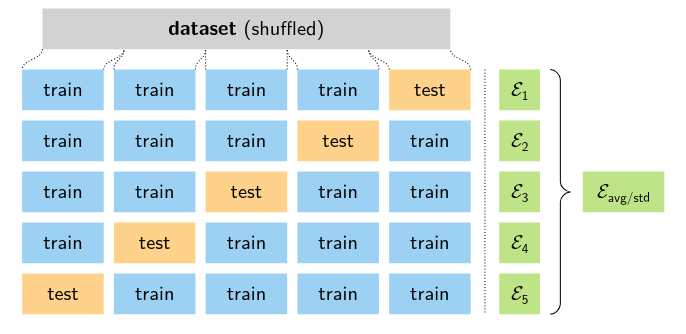
\includegraphics[width=7cm]{crossval}
	\end{center}
\end{wrapfigure}
If by splitting data evenly into a training and test set there is not much data left for both procedures, we get worse models and noisier error estimates. This can be addressed by cross-validation: repeating the analysis over \textbf{multiple splits} and \textbf{averaging} the results. Since this operation reduces the noise of error estimates, most of data should be allocated fro training ($80\%$).

\paragraph{Overfitting} This phenomena causes models that perform better on the training set to do worse on the test one. This is due to the model trying to extract more variations that can possibly be recovered from the input features, lowering the training error but performing worse on out-of-sample data.
\begin{center}
	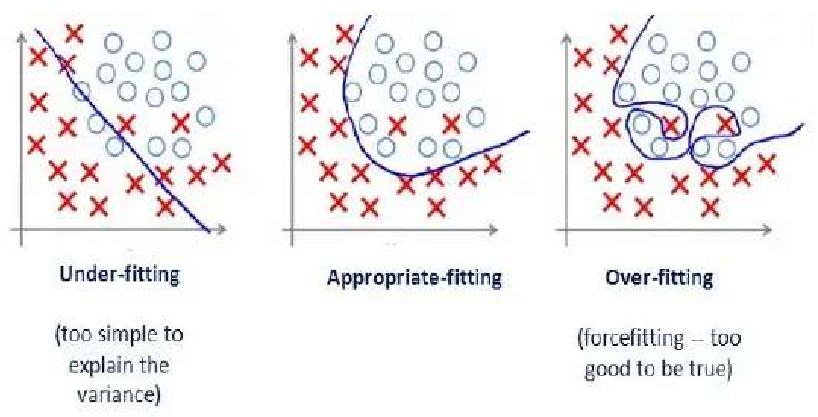
\includegraphics[scale=.4]{overfit}
\end{center}

\subsection{Modeling complexity}
\begin{wrapfigure}[7]{r}{6cm}
	\vspace{-.9cm}
	\begin{center}
		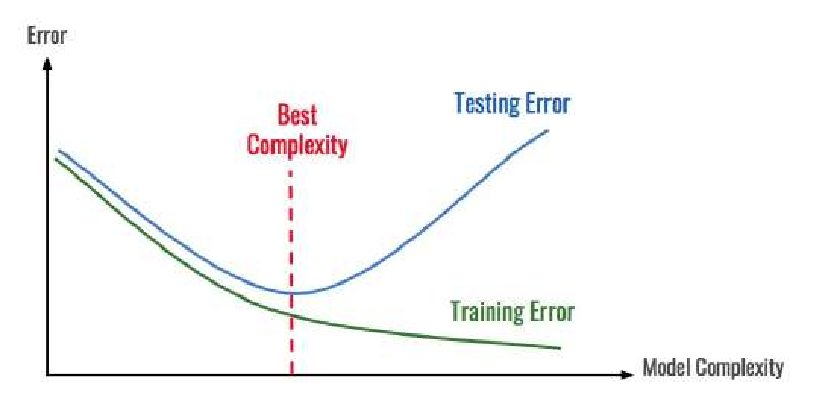
\includegraphics[width=6cm]{modelcomp}
	\end{center}
\end{wrapfigure}
By controlling the complexity of a model, one can reach a good trade off between \textbf{underfitting} and \textbf{overfitting}, hence performing better on the test data.\\

To do this we need a mechanism within the learning procedure to control model complexity so that we can adjust it. There are two approaches:
\begin{itemize}
	\item \textbf{Feature selection}: define a limited set of features $\mathcal{I}$, with $\lvert\mathcal{I}\rvert < d$, that the model can use for training
	\item \textbf{Model regularization}: penalize models that are oversensitive to small variations of the data, e.g. for a linear model impose $\lvert\lvert \mathbf{w}\rvert\rvert^2 < R$ on the weight. The lower the \textit{hyperparameter} R, the less likely to overfit
\end{itemize}

\subsubsection{Least Square Regression}
To regularize LSR we proceed in two steps:
\begin{enumerate}
	\item Build the Lagrangian
	\begin{equation*}
		\mathcal{L}(\mathbf{w}, \lambda) = \frac{1}{2} \mathbb{E}[\lvert\lvert\mathbf{w}^\top\mathbf{x}-y\rvert\rvert^2] + \frac{1}{2}\lambda(\lvert\lvert \mathbf{w} \rvert\rvert^2-S)
	\end{equation*}
	\newpage
	\item Verify Slater's conditions and apply the KKT conditions:
	\begin{itemize}
		\item \textbf{Stationarity} gives us:
		\begin{equation*}
			\frac{\nabla\mathcal{L}}{\nabla\mathbf{w}} = \underbrace{\mathbb{E}[\mathbf{x}\mathbf{x}^\top]}_{C_{xx}}\mathbf{w} - \underbrace{\mathbb{E}[\mathbf{x}y]}_{C_{xy}} + \lambda\mathbf{w} \overset{\text{def}}{=} \mathbf{0}
		\end{equation*}
		and therefore
		\begin{equation*}
			\mathbf{w} = (C_{xx}+\lambda I)^{-1}C_{xy}
		\end{equation*}
		\item \textbf{Complementary slackness} gives us:
		\begin{equation*}
			\lambda \cdot (\lvert\lvert \mathbf{w}\rvert\rvert^2 - S) = 0
		\end{equation*}
		If $\lambda > 0$ then $\lvert\lvert \mathbf{w}\rvert\rvert^2=S$. If $\lvert\lvert \mathbf{w}\rvert\rvert^2<S$ then $\lambda=0$ (standard regression).
	\end{itemize}
\end{enumerate}

\begin{center}
	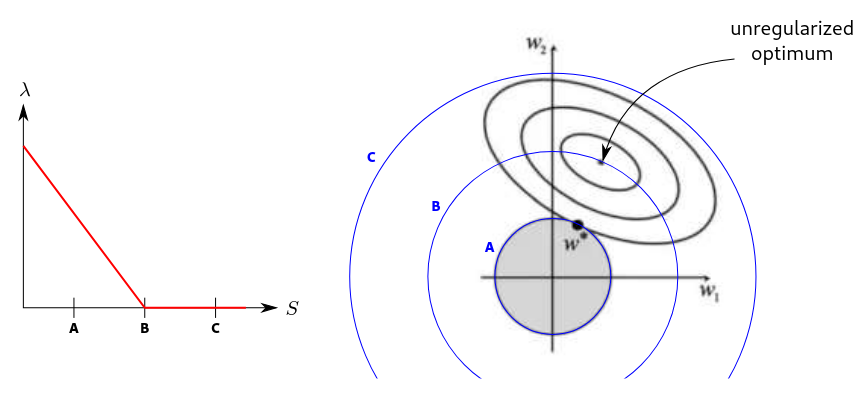
\includegraphics[scale=.4]{reglsr}
\end{center}

\begin{observation}
	Since we want to try many parameter $S$, we should not try to resolve $\lambda$ from it but instead try different parameters $\lambda$ too.
\end{observation}

\subsubsection{Fisher Discriminant}
Like with the Least Square Regression, the Fisher discriminant can be expressed with regularization as:
\begin{equation*}
	\mathbf{w} = (C_{xx}+\lambda I)^{-1}(\mu_2 - \mu_1)
\end{equation*}
Increasing $\lambda$ makes the inverse covariance term more similar to an identity and the direction $\mathbf{w}$ becomes aligned with that of the difference of means ($\mathbf{w} = \mu_2-\mu_1$).
\begin{center}
	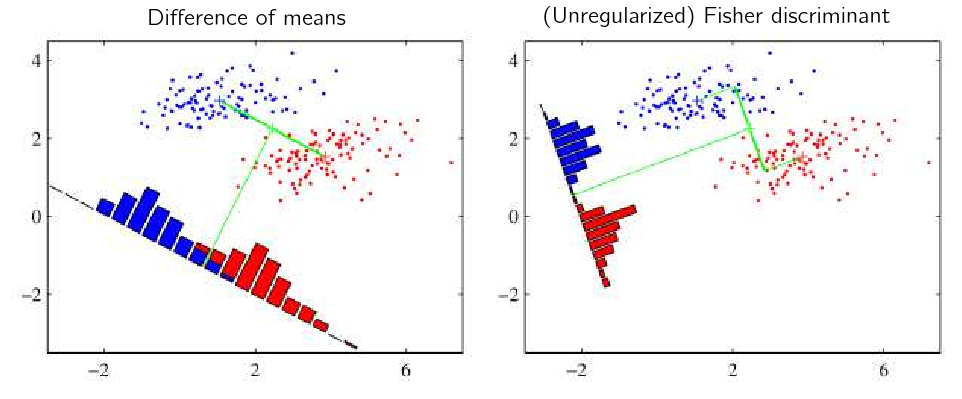
\includegraphics[scale=.4]{fisherreg}
\end{center}

\subsection{Vapnik-Chervonenkis Theory}
Now we want to formally connect model complexity to the true (\textit{reproducible}) error of a model.\\

We can define the true error, given a ground-truth joint distribution $p(\mathbf{x},y)$ over the input $\mathbf{x} \in \mathbb{R}^d$ and the output $y \in \mathbb{R}^d$, of some predictor $f: \mathbb{R}^d \to \mathbb{R}$ by the integral:
\begin{equation}
	\varepsilon_\text{true}(f) = \int \ell(f(\mathbf{x}),y)dp(\mathbf{x},y)
\end{equation}
where $\ell(f(\mathbf{x}),y)$ is some \textbf{loss function}. In practice $p$ is unknown and therefore we only know the \textit{train} error:
\begin{equation}
	\varepsilon_\text{train}(f) = \frac{1}{N} \sum_{i=1}^{N}\ell(f(\mathbf{x}_i), y_i)
\end{equation}

Vapnik-Chervonenkis theory provide a connection between training and true error in the context of classification. Specifically, it shows that with probability $1 - \delta$:
\begin{equation}
	\varepsilon_\text{true}(f) - \varepsilon_\text{train}(f) \leq \sqrt{\frac{h_\mathcal{F} \cdot \bigg(\log\bigg(\frac{2N}{h_\mathcal{F}}\bigg)+1\bigg)-\log\bigg(\frac{\delta}{4}\bigg)}{N}}
\end{equation}
where $h_\mathcal{F}$ is the VC \textbf{dimension} measuring the complexity of the class models $\mathcal{F}$ which ours is selected from. Specifically, the maximum number of data points that the class can always classify in any possible way. Some examples are:
\begin{itemize}
	\item $
		f(\mathbf{x}) = \text{sign}(\sin(\mathbf{w}^\top \mathbf{x}+b)) \qquad\qquad\qquad\qquad h_\mathcal{F} = \infty
$
	\item $
		f(\mathbf{x}) = \text{sign}(\mathbf{w}^\top \mathbf{x}+b) \qquad\qquad\qquad\qquad\qquad h_\mathcal{F} = d+1
$
	\item $
		f(\mathbf{x}) = \text{sign}(\mathbf{w}^\top \mathbf{x}+b)\qquad \frac{1}{\lvert\lvert \mathbf{w} \rvert\rvert} = \frac{M}{2} \qquad\qquad h_\mathcal{F} \leq \min\{d+1, \lceil \frac{4r^2}{M^2} \rceil +1\}
$
\end{itemize}
\end{document}
